\subsection{ROUGE}
\begin{table}[h]
\centering
% centering table
\begin{tabular}{l c c c}
% creating 10 columns
\multicolumn{4}{c}{ROUGE-1}\\
\hline
\hline
% inserting double-line
$\mathrm{System}$ & $\mathrm{Recall}$ & $\mathrm{Prec.}$ & $\mathrm{F}_1$\\
[0.5ex]
\hline
AP+Salience & $\mathbf{0.282}$ & $\mathbf{0.344}$ & $\mathbf{0.306}$ \\
AP          & $0.245$ & $0.285$ & $0.263$ \\
RS          & $0.230$ & $0.271$ & $0.247$ \\
HAC         & $0.169$ & $0.230$ & $0.186$ \\
\hline % inserts single-line
\end{tabular}
~\\[1ex]
~\\
\begin{tabular}{l c c c}
% creating 10 columns
\multicolumn{4}{c}{ROUGE-2}\\
\hline
\hline
% inserting double-line
$\mathrm{System}$ & $\mathrm{Recall}$ & $\mathrm{Prec.}$ & $\mathrm{F}_1$\\[0.5ex]
\hline
AP+Salience & $\mathbf{0.045}$ & $\mathbf{0.056}$ & $\mathbf{0.049}$ \\
AP          & $0.033$ & $0.038$ & $0.035$ \\
RS          & $0.031$ & $0.037$ & $0.034$ \\
HAC         & $0.017$ & $0.024$ & $0.019$ \\
\hline % inserts single-line
\end{tabular}
%~\\[1ex]
%~\\
%\begin{tabular}{l c c c}
%% creating 10 columns
%\multicolumn{4}{c}{ROUGE-L}\\
%\hline
%\hline
%% inserting double-line
%$\mathrm{System}$ & $\mathrm{Recall}$ & $\mathrm{Prec.}$ & $\mathrm{F}_1$\\[0.5ex]
%\hline
%AP+Salience & $0.275$ & $0.336$ & $0.299$ \\
%AP          & $0.241$ & $0.280$ & $0.258$ \\
%RS          & $0.225$ & $0.265$ & $0.242$ \\
%HAC         & $0.166$ & $0.225$ & $0.182$ \\
%\hline % inserts single-line
%\end{tabular}
%
%
\caption{System ROUGE performance.} % title name of the table
\label{tab:rouge}
\end{table}






Table~\ref{tab:rouge} shows our results for system output samples against the 
full summary of nuggets using ROUGE. This improvement is statistically 
significant for all ngram precision, recall, and F-measures at the 
$\alpha = .01$ level using the Wilcoxon signed-rank test. 


\begin{figure}
    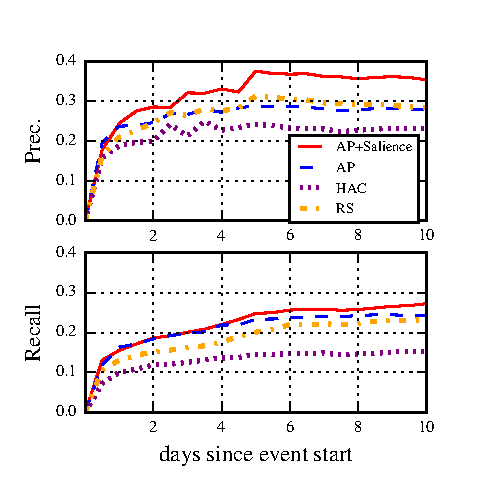
\includegraphics[]{rouge-time.eps}
\caption{System ROUGE-1 performance over time.}
\label{fig:trouge}
%\vspace{-14pt}
\end{figure}


\textsc{AP+Salience} maintains its performance above the baselines over time 
as well. Figure~\ref{fig:trouge} shows the ROUGE-1 scores over time. We show 
the difference in unigram precision (bigram precision is not shown but it 
follows similar curve). Within the initial days of the event, 
\textsc{AP+Salience} is able to take the lead over the over systems in ngram 
precision. The \textsc{AP+Salience} model is better able to find salient 
updates earlier on; for the disaster domain, this is an especially important 
quality of the model. 


Moreover, the \textsc{AP+Salience}'s recall is not diminished by the high 
precision and remains competitive with \textsc{AP}. Over time 
\textsc{AP+Salience}'s recall also begins to pull away, while the other models
start to suffer from topic drift.


\subsection{Expected Gain and Comprehensiveness}
\begin{figure}[h]
  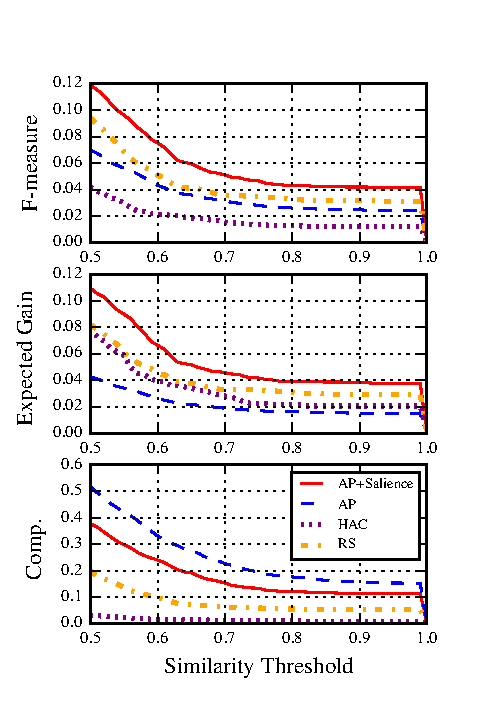
\includegraphics[]{nuggets-metrics2.eps}
\caption{Expected Gain and Comprehensiveness performance.}
\label{fig:nperf}
%\vspace{-12pt}
\end{figure}


Figure~\ref{fig:nperf} shows the expected gain across a range of similarity 
thresholds, where thresholds closer to 1 are more conservative estimates. 
The ranking of the systems remains constant across the sweep with 
\textsc{AP+Salience} beating all baseline systems. Predicting salience in 
general is helpful for keeping a summary on topic as the \textsc{RS} approach 
out performs the clustering only approaches on expected gain.


When looking at the comprehensiveness of the summaries \textsc{AP} outperforms
\textsc{AP+Salience}. The compromise encoded in the \textsc{AP+Salience} 
objective function, between being representative and being salient, is seen 
clearly here where the performance of the \textsc{AP+Salience} methods is 
lower bounded by the salience focused \textsc{RS} system and upper bounded by 
the clustering only \textsc{AP} system. Overall, \textsc{AP+Salience} achieves
the best balance of these two metrics.


\subsection{Feature Ablation}
\begin{table}[h]
\centering
% centering table
\begin{tabular}{l c c c}
% creating 10 columns
\multicolumn{4}{c}{ROUGE-1}\\
\hline
\hline
% inserting double-line
$\mathrm{System}$ & $\mathrm{Recall}$ & $\mathrm{Prec.}$ & $\mathrm{F}_1$\\
[0.5ex]
\hline
Full System & $0.282$ & $0.344$ & $0.306$ \\
No Basic    & $0.263$ & $0.380^\dagger$ & $0.294$ \\
No LM       & $0.223^\dagger$ & $0.361$ & $0.254^\dagger$ \\
No Time  & $0.297^\dagger$ & $0.367^{\dagger\dagger}$ & $0.322^\dagger$ \\ 
No Geo   & $0.232^{\dagger\dagger}$ & $0.381$ & $0.265^\dagger$ \\  
No Query & $0.251$ & $0.377$ & $0.280$ \\ 
\hline % inserts single-line
\end{tabular}
~\\[1ex]
~\\
\begin{tabular}{l c c c}
% creating 10 columns
\multicolumn{4}{c}{ROUGE-2}\\
\hline
\hline
% inserting double-line
$\mathrm{System}$ & $\mathrm{Recall}$ & $\mathrm{Prec.}$ & $\mathrm{F}_1$\\[0.5ex]
\hline
Full System & $0.045$ & $0.056$ & $0.049$ \\
No Basic    & $0.046$ & $0.068^{\dagger\dagger}$ & $0.051^\dagger$ \\
No LM       & $0.033^\dagger$ & $0.056$ & $0.038^\dagger$ \\
No Time  & $0.052^{\dagger\dagger}$ & $0.064^{\dagger\dagger}$ & $0.056^{\dagger\dagger}$ \\
No Geo   & $0.037^\dagger$ & $0.065$ & $0.042$ \\
No Query & $0.043$ & $0.068^\dagger$ & $0.048$ \\
\hline % inserts single-line
\end{tabular}
\caption{Feature ablation ROUGE performance. 
    $\dagger$ indicates statistically significant difference from 
full model at the $\alpha=.05$ level.
    $\dagger\dagger$ indicates statistically significant difference from 
full model at the $\alpha=.01$ level.
    } % title name of the table
\label{tab:farouge}
\end{table}









Table~\ref{tab:farouge} shows the results of our feature ablation tests. 
Removing the language models yields a statistically significant drop in both 
ngram recall and F-measure. Interestingly, removing the basic features leads 
to an increase in both unigram and bigram precision; in the bigram case this 
is enough to cause a statistically significant increase in F-measure over the 
full model. In other words, the generic features actually lead to an inferior 
model when we can incorporate more appropriate domain specific features.
The result mirrors Sparck Jones' claim that generic approaches to 
summarization cannot produce a useful summary \cite{ksj98}.


\begin{figure*}
%\begin{tabular}{|l m{15cm}|}
%\multicolumn{2}{c}{\textbf{Hurricane Sandy}}\\
%\hline
%\hline
%%\small
%%\tabitem The forecast map shows Sandy reaching eastern Cuba by early Thursday 
%%    before heading to the Bahamas.\\
%%\small
%%\tabitem Jamaica's government issued a hurricane warning on Tuesday morning and 
%%    announced schools would be closed on Wednesday.\\
%\small
%\tabitem  & \small Dangerous flash floods and mudslides set off by Sandy were a threat for the
%   island of roughly 2.7 million inhabitants, Jamaica's meteorological service
%   said.\\
%\small
%\tabitem  & \small A few reliable forecast models bring Sandy close enough to the coast to 
%   produce heavy rains, strong winds and beach erosion.\\
%\small
%\tabitem  & \small Max winds are 65 mph with strengthening to a hurricane expected in the next
%   12 to 18 hours.\\
%\small
%\tabitem & \small The two international airports, as well as schools and businesses, 
%         will remain closed today until the hurricane warning, which is now in
%         effect for the island, is lifted. \\
%\hline
%%at 11 a.m., sandy was in the caribbean about 65 miles south of kingston , jamaica , moving north at 13 mph with sustained winds of 80 mph.
%%"""""""we heard on the radio that the hurricane was coming this way,"""""""" he said in the poor kingston community of standpipe, situated next to one of the debris-clogged gullies that crisscross the capital."""""""
%\end{tabular}
%
%~\\
%~\\
\begin{tabular}{|l m{15cm}|}
\multicolumn{2}{c}{\textbf{2012 Pakistan Garment Factory Fires}}\\
\hline
\hline
%\small
%\tabitem Medical officials said that some had died of suffocation while others
%         were burnt alive as the fire took hold. \\
\small
\tabitem & \small The fire broke out when people in the building were trying to start 
         their generator after the electricity went out. \\
\small
\tabitem & \small Pakistani television showed pictures of what appeared to be a 
         three-story building with flames leaping from the top-floor windows 
         and smoke billowing into the night sky. \\
\small
\tabitem & \small The people went to the back side of the building but there was no 
         access, so we had to made forceful entries and rescue the people, 
         said Numan Noor, a firefighter on the scene. \\
\small
\tabitem & \small ``We have recovered 63 bodies, including three found when we reached 
         the basement of the building,'' Karachi fire chief Ehtesham Salim told
         AFP on Wednesday. \\
%\small
%\tabitem Salim added that the blaze was Karachi’s ``biggest fire in terms of 
%         deaths in decades.'' \\
%\small
%\tabitem The garment trade as a whole is vital to Pakistan’s shaky economy. \\
\hline
\end{tabular}

~\\
~\\
\begin{tabular}{|l m{15cm}|}
\multicolumn{2}{c}{\textbf{2012 Romanian Protests}}\\
\hline
\hline
\small
\tabitem & \small Clashes between riot police and demonstrators have also erupted in 
         the Romanian capital Bucharest for a third day in a row. \\
\small
\tabitem & \small BOC urged Romanians to understand that tough austerity measures are 
         needed to avoid a default. \\
\small
\tabitem & \small More than 1,000 protesters rallied in Bucharest's main university 
         square, blocking traffic. \\
\small
\tabitem & \small Bucharest : a Romanian medical official says 59 people suffered 
         injuries as days of protests against the government and austerity 
         measures turned violent. \\
%\small
%\tabitem Most Romanians agree that only fundamental reform can save the 
%         country's ailing and corrupt system. \\
%\small
%\tabitem Many Romanians feared this would only increase corruption and create 
%         a further divide between the classes, leading to a two-tier system in
%         which only the wealthy would be able to afford care. \\
\hline
\end{tabular}

\caption{\textsc{AP+Salience} summary excerpts.}
\label{fig:summaries}
\end{figure*}



Removing the language model and geographic relevance features leads to a
statistically significant drop in ROUGE-1 F1 scores. Unfortunately,
this is not the case for the temporal relevance features. We surmise that
these features are too strongly correlated with each other, 
i.e. the differences in TF*IDF between hours are definitely not i.i.d. 
variables. 
